\documentclass[12pt]{article}
\title{ECE 141 Homework 2}
\usepackage{subcaption}
\author{Lawrence Liu}
\usepackage{graphicx}
\usepackage{amsmath}
\usepackage{placeins}
\newcommand{\Laplace}{\mathscr{L}}
\setlength{\parskip}{\baselineskip}%
\setlength{\parindent}{0pt}%
\usepackage{xcolor}
\usepackage{listings}
\definecolor{backcolour}{rgb}{0.95,0.95,0.92}
\usepackage{amssymb}
\lstdefinestyle{mystyle}{
    backgroundcolor=\color{backcolour}}
\lstset{style=mystyle}

\begin{document}
\maketitle
\section*{Problem 6.5}

This has two break points, one at $\omega=1$ and another at $\omega=2$. Furthermore because of the $\frac{1}{s}$, we
have that the sketch of the bode plots look like.\\
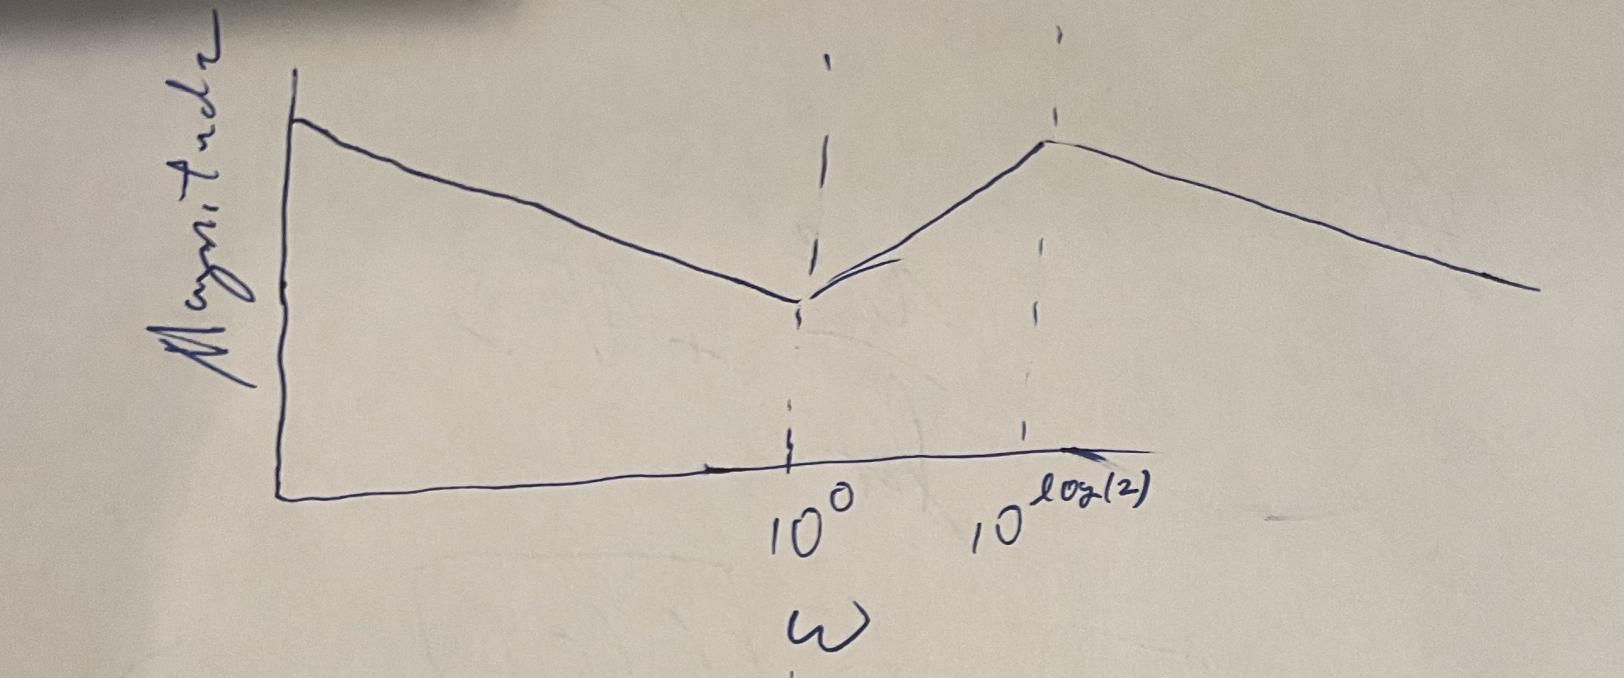
\includegraphics[scale=0.2]{Problem1Fig1.png}\\
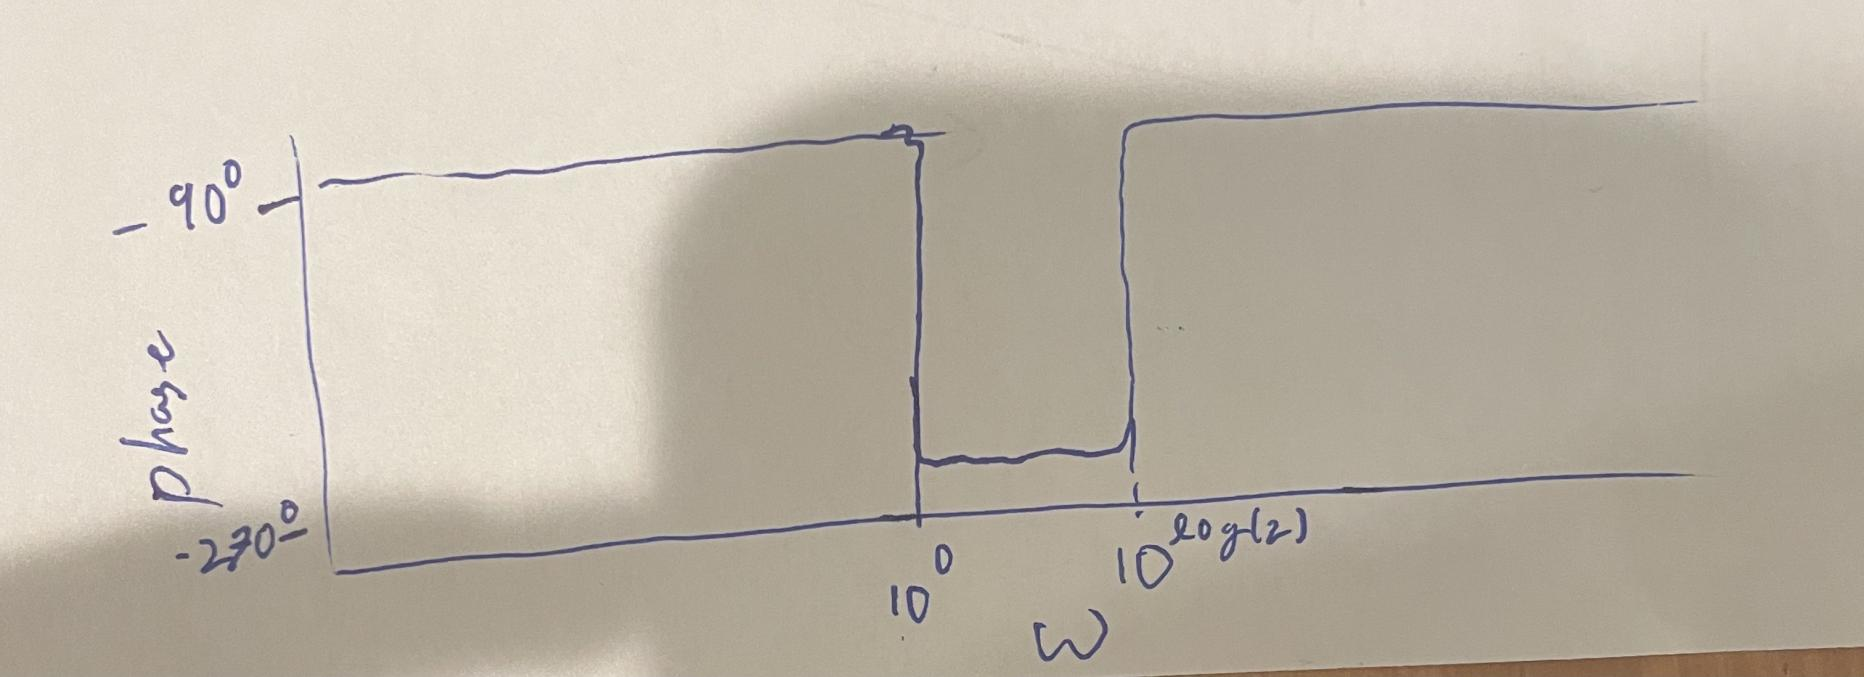
\includegraphics[scale=0.2]{Problem1Fig2.jpg}\\
We can confirm this with the following matlab code
\begin{verbatim}
sys = tf([1 0 4], [1 0 1 0]);
bode(sys)
\end{verbatim}
Which outputs the following plot\\
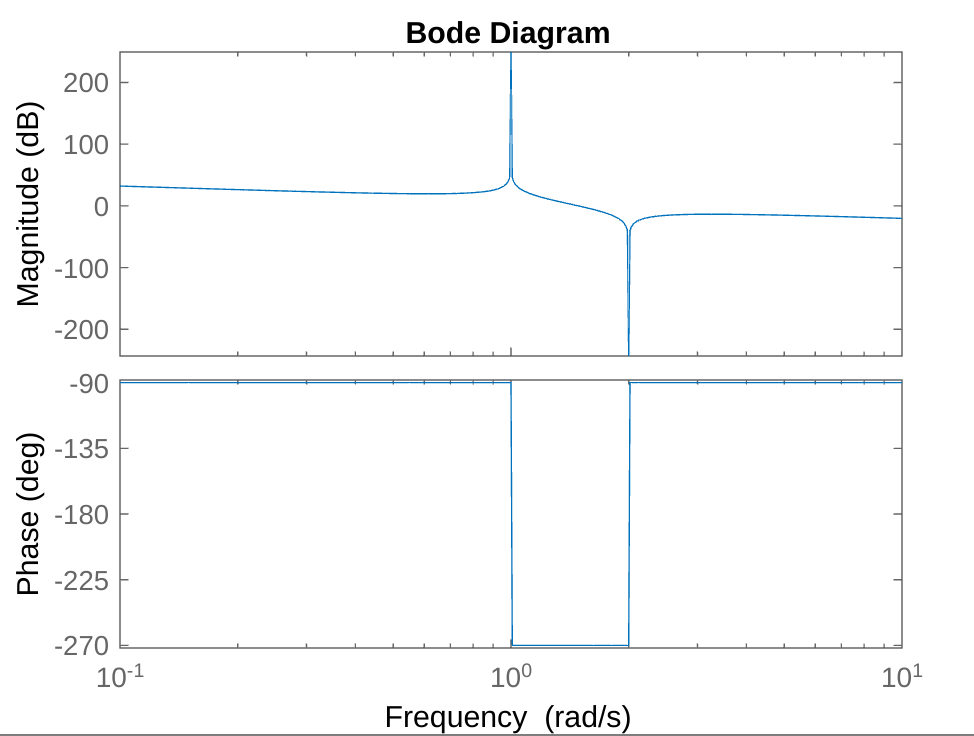
\includegraphics[scale=0.2]{Problem1Fig3.png}\\
\section*{Problem 6.7}
There are 3 break points, one first order one at $\omega=2$ in the numerator, one second order one at $\omega=5$ in the denominator and a first order one at $
\omega=10$ in the denominator. Furthermore since there also exists a $s^2$ in the denominator, we start of initially with a slope of $-2$. Therefore, we can
the sketch of the bode plot looks like.\\
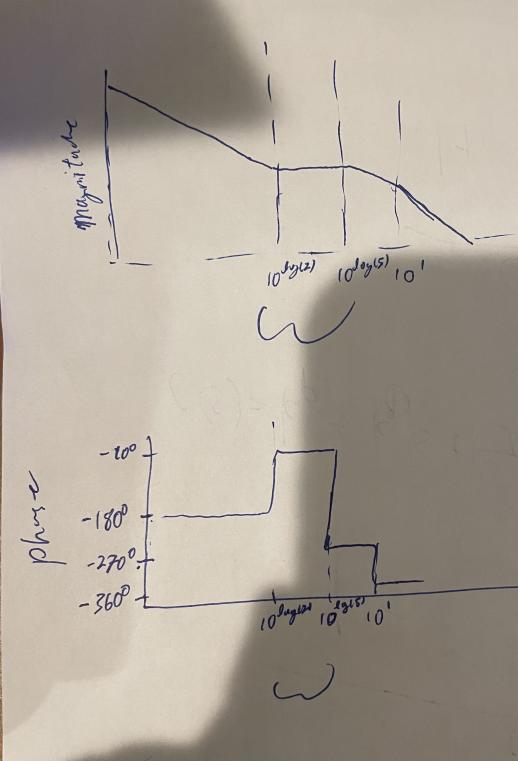
\includegraphics[scale=0.4]{Problem2Fig1.jpg}\\
We can confirm this with the following matlab code
\begin{verbatim}
u = [1 10];
v = [1 0 0];
y=[1 6 25];

conv(conv(u,v),y)

sys = tf([1 2], conv(conv(u,v),y));
bode(sys)
\end{verbatim}
Which outputs the following plot\\
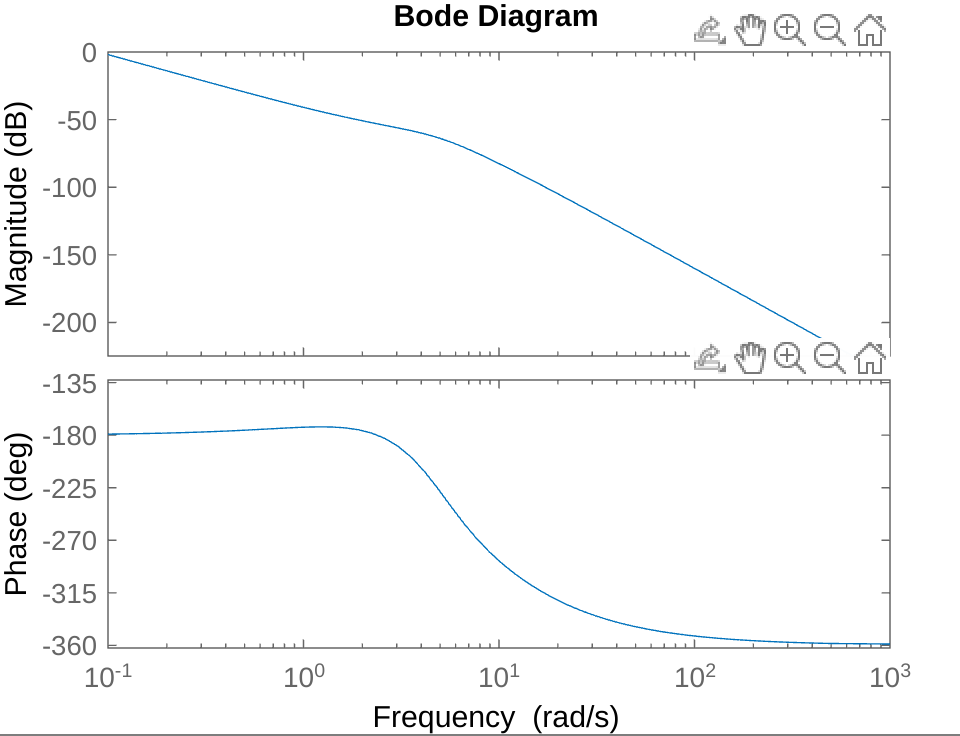
\includegraphics[scale=0.2]{Problem2Fig2.png}\\
\section*{Problem 6.16}
through this matlab code we get the following bode plot
\begin{verbatim}
u = [1 10];
v = [1 1];


conv(conv(u,v),v)

sys = tf([1], conv(conv(u,v),v));
[mag,phase,wout] = bode(sys)
\end{verbatim}
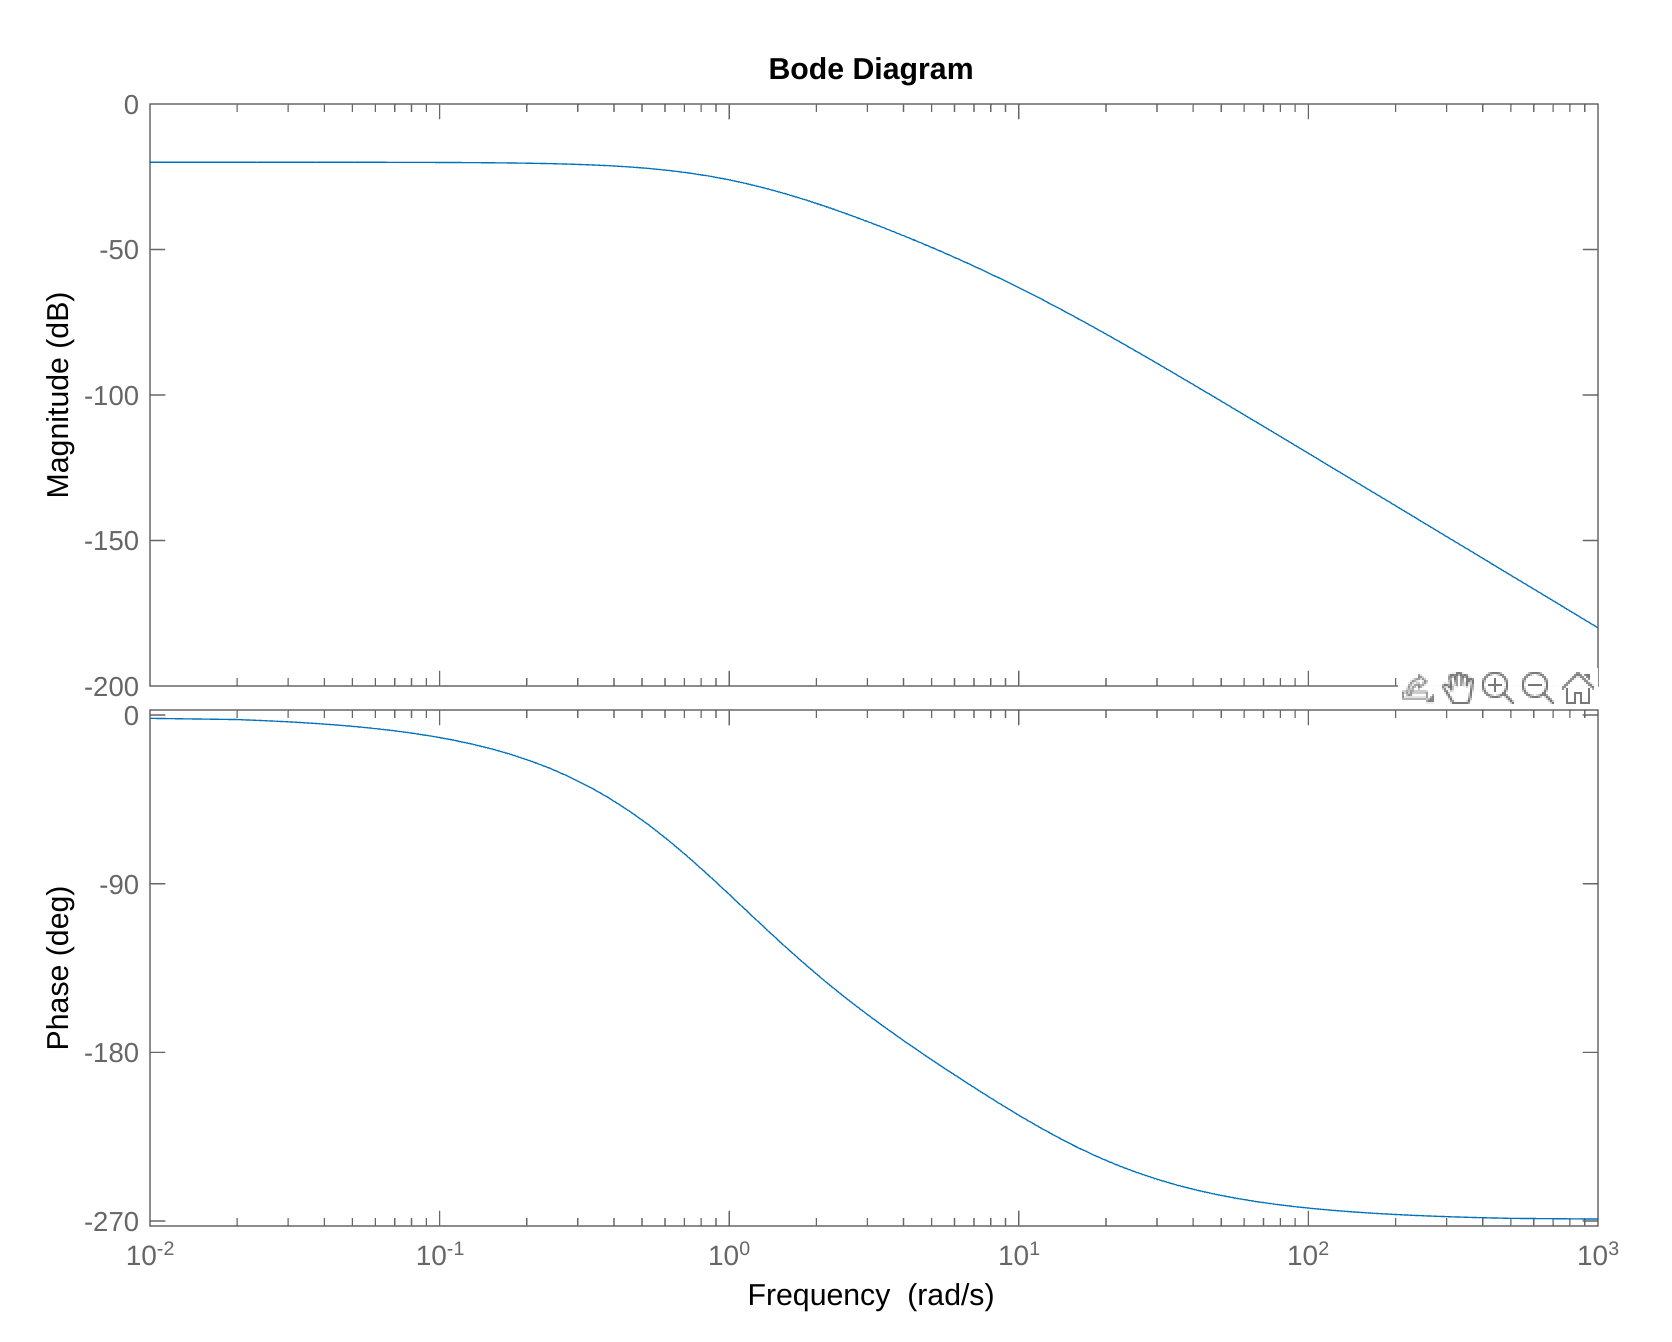
\includegraphics[scale=0.2]{Problem3Fig1.png}\\
Therefore, with the following matlab code we find that $K<251.5348$ for stability
\begin{verbatim}
m=mag(phase<-180);
1/max(m)
\end{verbatim}
We can confirm this by plotting out the root locus, we have that there are 3 poles, 2 at -1, and 1 at -10, with angles of departure of $\pm90^{circ}$ and $180^{\circ}$.
 $\alpha=4$, the assympotic angles are $\pm60^{\circ}$ and $180^{\circ}$.
 Therefore the root locus looks like\\
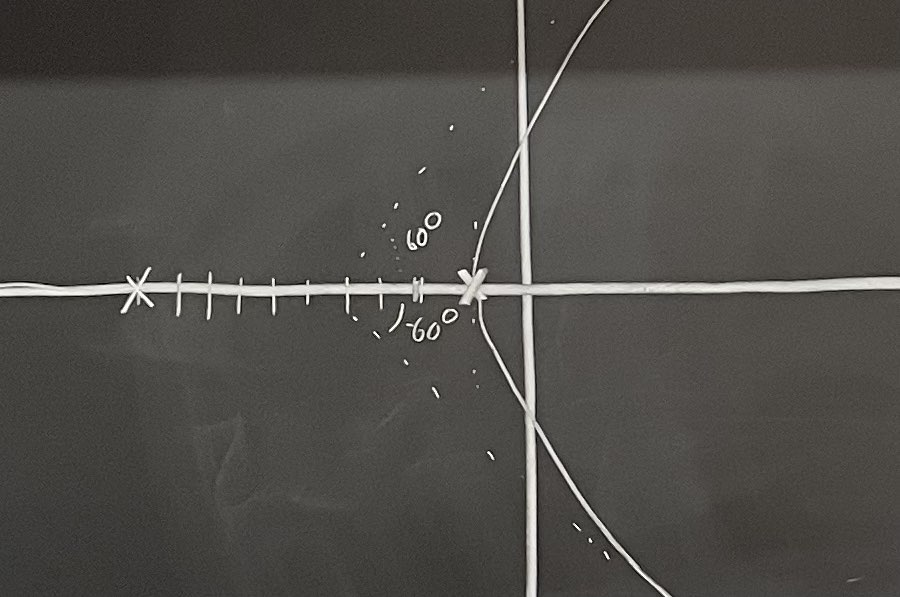
\includegraphics[scale=0.4]{Problem3Fig2.jpg}\\
\section*{Problem 6.17}
Plotting out the bode plot with the following code
\begin{verbatim}
u = [1 0 9];
v = [1 2];


conv(u,v)

sys = tf([1], conv(u,v));
bode(sys)
\end{verbatim}
which yields the following bode plot\\
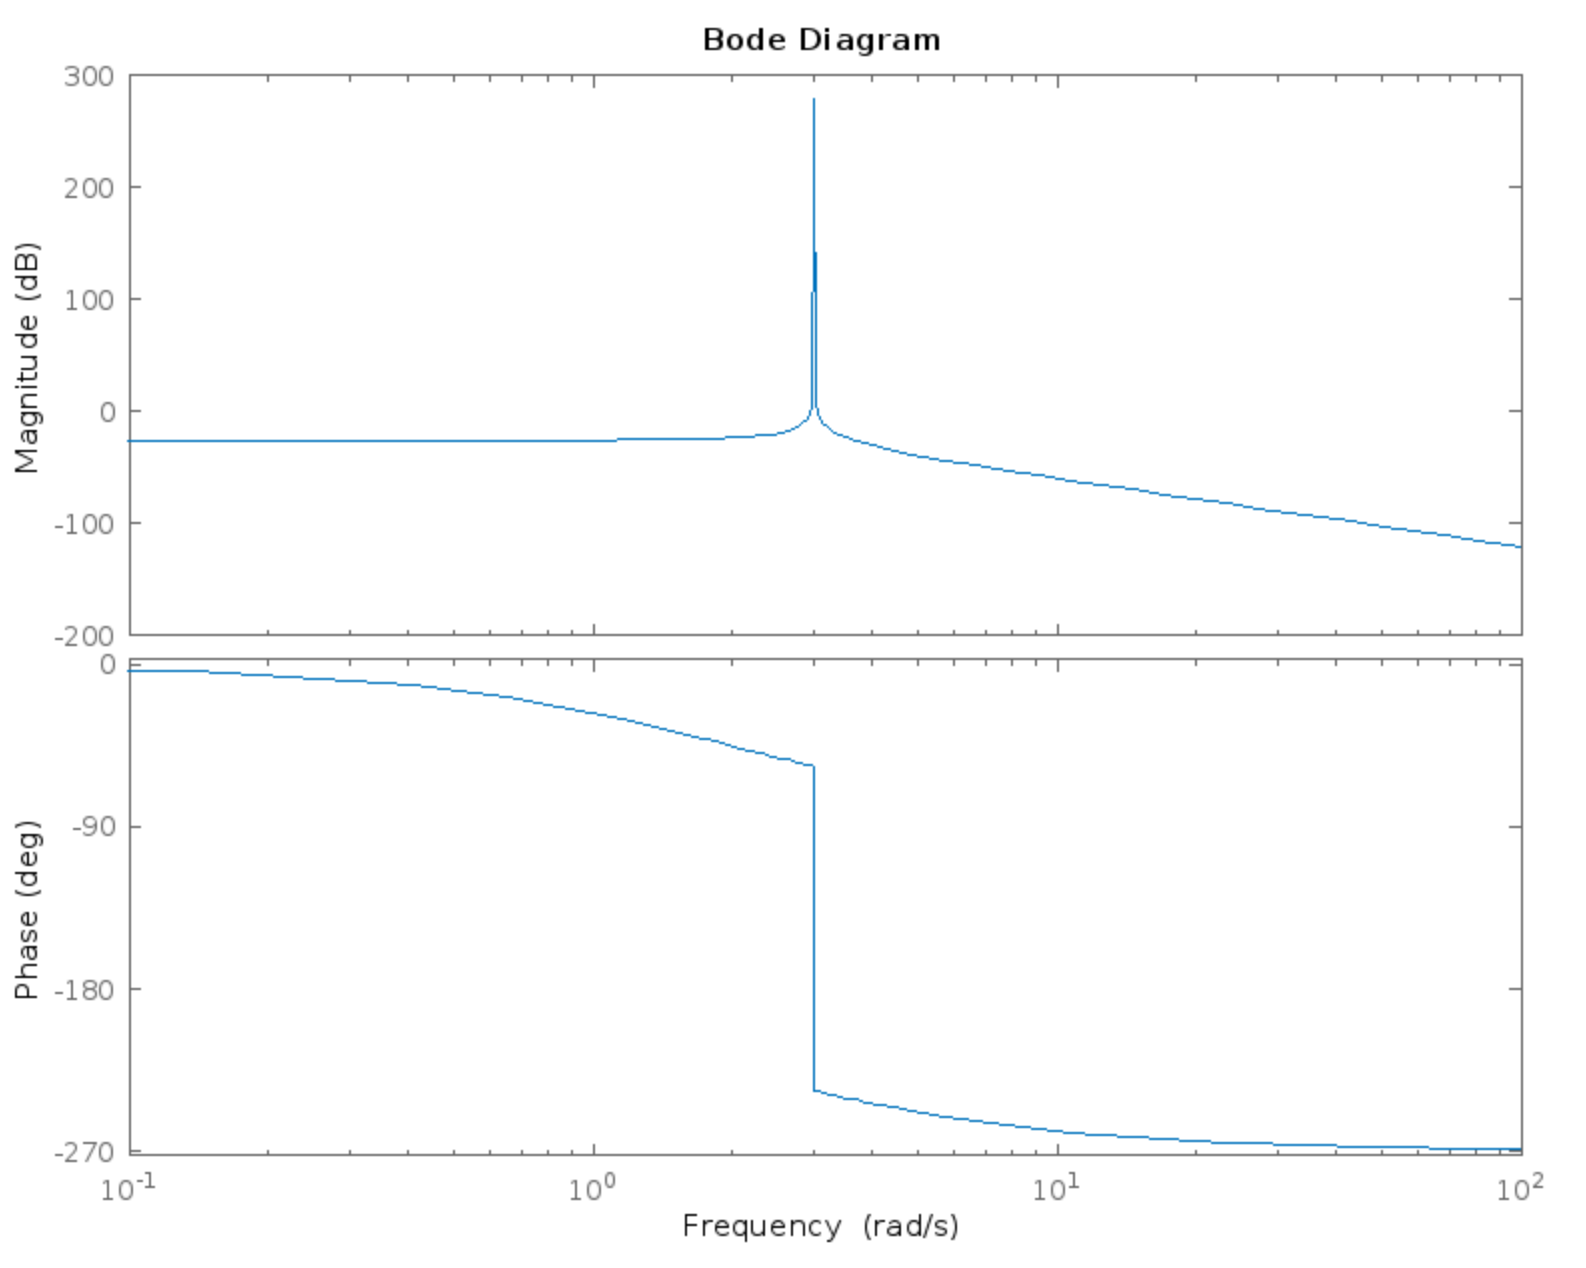
\includegraphics[scale=0.2]{Problem4Fig1.png}
There is a spike at $\omega=3$, therefore there is a spike to infity at that point, furthermore, the phase will change by $-180^{\circ}$ at that point. Therefore no values of $K$ can
make the system stable, we can confirm this by plotting out the root locus, we have that there are 3 poles, 2 at $\pm 3j$ and one at $-2$, the angles of departure from these poles are
$\pm33.69^{\circ}$ and $180^{\circ}$ respectively, furthermore $\alpha=\frac{2}{3}$, the assympotic angles are $\pm60^{\circ}$ and $180^{\circ}$.
 Therefore the root locus looks like\\
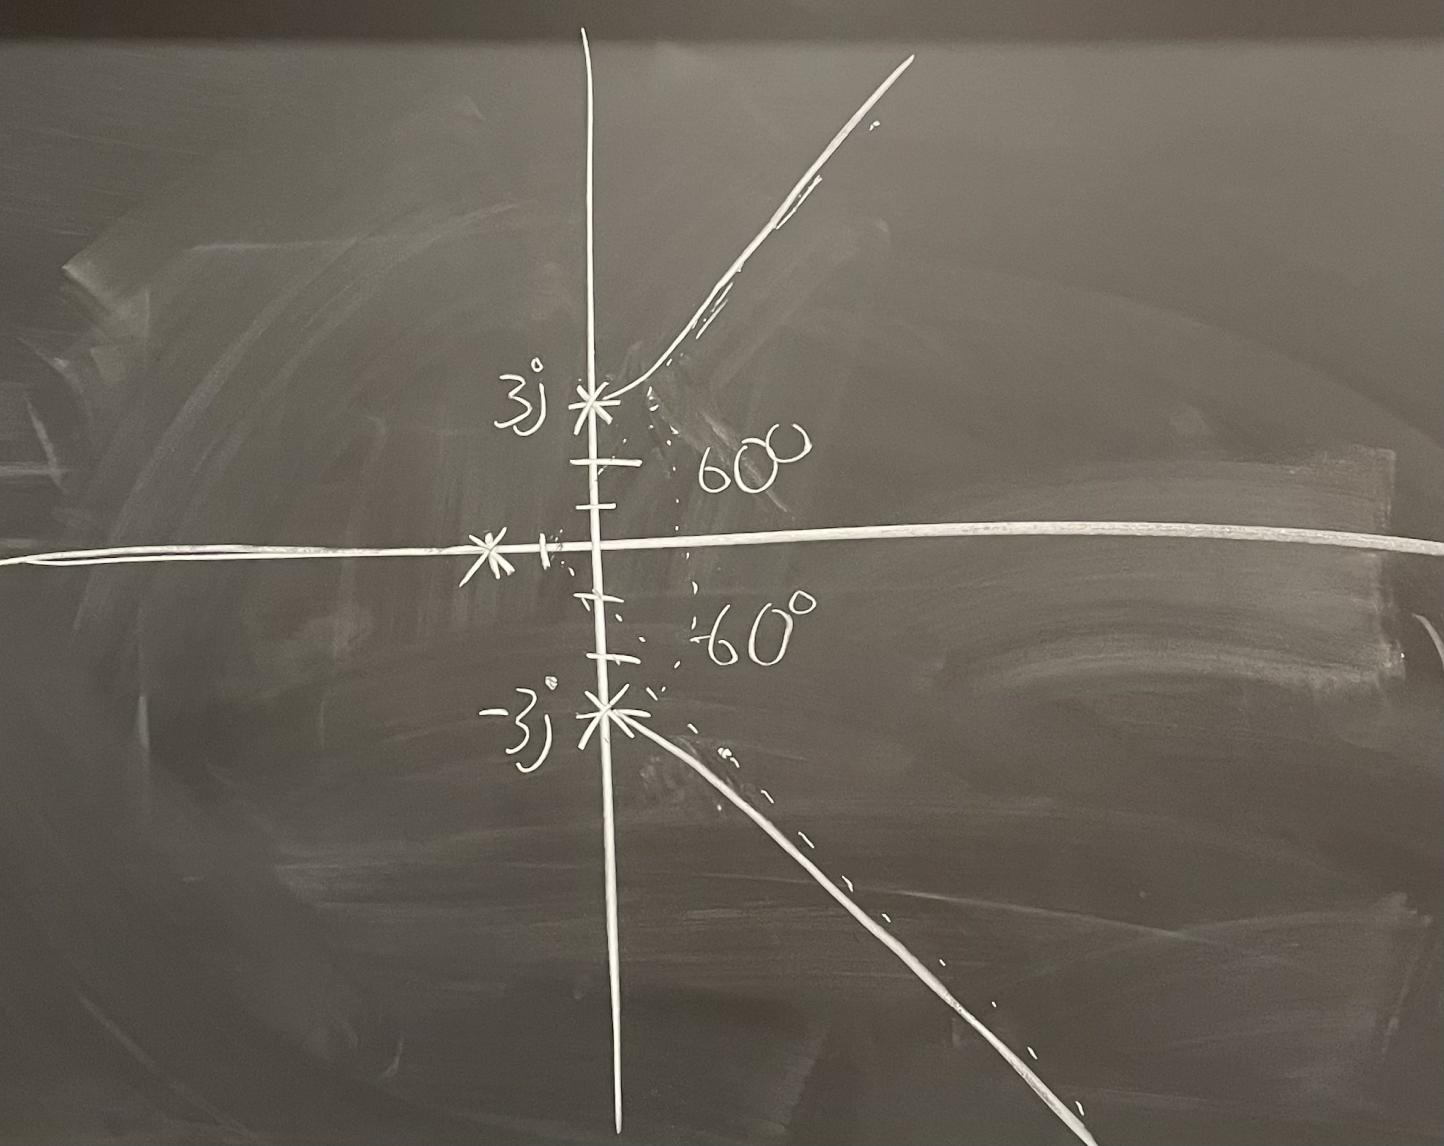
\includegraphics[scale=0.2]{Problem4Fig2.jpg}

\end{document}